\begin{frame}[noframenumbering,plain]
    \setcounter{framenumber}{1}
    \maketitle
\end{frame}


\begin{frame}
    \frametitle{Цели диссертации}
Целью данной работы является определение закономерностей, влияющих на перенос знаний между языками и задачами в многозадачных нейросетевых моделях на различных архитектурах и определение закономерностей, влияющих на особенности прикладного применения этих моделей в диалоговых платформах.
\end{frame}

\begin{frame}
\frametitle{Задачи диссертации}
Для достижения поставленной цели требовалось решить следующие задачи:
\begin{enumerate}
  \item {Определить закономерности переноса знаний при псевдоразметке данных для многозадачных нейросетевых моделей с одним линейным слоем.}
  \item {Определить закономерности переноса знаний в энкодер-агностичных многозадачных нейросетевых моделях между различными диалоговыми задачами. Провести оценку зависимости этого переноса от размера обучающей выборки.}
  \item {Определить закономерности переноса знаний в многоязычных энкодер-агностичных многозадачных нейросетевых моделях между различными языками -- с английского языка на русский. Провести оценку зависимости этого переноса от размера обучающей выборки.}
  \item {Интегрировать энкодер-агностичные многозадачные нейросетевые модели в open-source библиотеку для решения задач машинного обучения.} 
\end{enumerate}
\end{frame}

\begin{frame}
\frametitle{Задачи диссертации}
\begin{enumerate}
\setcounter{enumi}{4}
  \item {Проверить зависимость межъязыкового переноса знаний на разговорных данных в многоязычных нейросетевых моделях от размера предобучающей выборки и генеалогической близости языков к языку дообучения.}
  %\item {Разработать компоненты диалоговой платформы, пригодные для изучения прикладного применения многозадачных нейросетевых моделей.} % TODO СПРОСИТЬ У ВАСИ
  \item {Интегрировать рассмотренные в диссертации многозадачные нейросетевые архитектуры в диалоговую платформу, оценить применимость данных архитектур и провести их сравнительный анализ на основании результатов на задачах данной платформы.}% todo программную библиотеку
\end{enumerate}
\end{frame}


\begin{frame}
\frametitle{Содержание работы}
\begin{enumerate}
    \item {Введение}
    \item {Нейросетевые методы машинного обучения для задач обработки естественного языка}
    \item {Использование псевдоразметки данных в многозадачных моделях для решения задач GLUE}
    \item {Энкодер-агностичные модели}
    \item {Исследование переноса знаний в многоязычных моделях на новом тематическом наборе данных}
    \item {Использование в диалоговой платформе {DeepPavlov Dream} многозадачных моделей}
\end{enumerate}
\end{frame}

\begin{frame}{0. Введение}
\begin{enumerate}
\item Модели типа BERT широко применяются.
\item Они требуют вычислительных мощностей - многозадачное обучение может помочь их сэкономить
\item Перенос знаний между задачами и языками не изучен до конца
\end{enumerate}
\end{frame}

\begin{frame}{1. Нейросетевые методы машинного обучения  для задач обработки естественного языка}
Вводятся базовые понятия глубокого обучения. В частности, поясняется принцип работы модели BERT и разбираются многозадачные архитектуры на её основе - PAL-BERT и MT-DNN. Даётся также определение переноса знаний.
\newline
\newline
Вывод - модели, основанные на описанных в данной главе нейросетевых архитектурах, пригодны для изучения многозадачного переноса знаний.
\end{frame}

\begin{frame}{2. Псевдоразметка данных: задача}
Определить закономерности переноса знаний при псевдоразметке данных для многозадачных нейросетевых моделей с одним линейным слоем. В таких моделях каждый нейрон последнего линейного слоя поверх трансформера может быть от 0 до 1 независимо от других нейронов.

    Для этого - исследовать разные способы псевдоразметки данных при обучении таких моделей(тело-BERT), на задачах из бенчмарка GLUE:
    \begin{enumerate}
    \item QQP -- задача классификации пар предложений из сайта Quora.com на 2 класса -- дубликат и не дубликат.
    \item MNLI -- задача классификации пар предложений из различных тем на три класса -- логическое следование, логическое противоречие и нейтральный(ни следование, ни противоречие).
    \item SST-2 -- задача классификации предложений на два класса -- положительная тональность и отрицательная тональность.
    \item RTE -- задача классификации пар предложений на два класса -- логическое следствие и нет логического следствия.
    \end{enumerate}
\end{frame}


\begin{frame}{2. Псевдоразметка данных: без объединения меток}
    \begin{enumerate}
\item \textbf{Независимые метки} -- метки для каждой задачи считаются независимыми (т.е всего 9 классов), каждый пример имеет метку 1 для того класса своей задачи, к которому он принадлежит и 0 для всех остальных классов всех остальных задач. 
\item \textbf{Независимые метки, замороженная голова} -- аналогично п.1, но линейный слой заморожен и обучается только тело модели.
\item \textbf{Мягкие независимые метки} -- аналогично п.1, но вероятности всех остальных классов каждой из остальных задач считаются равными друг другу так, чтобы их сумма равнялась 1. 
\item \textbf{Мягкие независимые метки, замороженная голова} -- аналогично п.3, но линейный слой заморожен и обучается только тело модели.
\item \textbf{Дополненные независимые метки} -- аналогичен п.3, но вероятности для всех классов каждой из остальных задач получаются при помощи предсказаний однозадачной модели, обученной исключительно на этой задаче.
    \end{enumerate}
\end{frame}


\begin{frame}{2. Псевдоразметка данных: с объединением меток}
    \begin{enumerate}
\item \textbf{Мягкое вероятностное предположение} -- объединение классов с сокращением их числа до пяти: положительный, отрицательный, логическое следствие, логическое противоречие, нейтральный. В остальном та же логика, что и для режима Мягкие независимые метки.
\item \textbf{Мягкие предсказанные метки} -- как \textbf{Дополненне независимые метки}, но с сокращением числа классов до пяти аналогично предыдущему пункту. 
\item \textbf{Жесткие предсказанные метки} -- аналогичен предыдущему, но для меток, полученных из предсказаний оригинальной модели, максимальная вероятность для каждой задачи округляется до 1, а все остальные вероятности до 0.
\item \textbf{Базовый} -- отдельный BERT для каждой задачи.
    \end{enumerate}
\end{frame}

\begin{frame}{2. Псевдоразметка данных: результаты}
\begin{table}[htbp]
\centering
\caption {Лучшая точность на тестовых данных (при лучшей скорости обучения из выбираемых, среднее по 3 запускам)}
\label{tab:ps2}% label всегда желательно идти после caption
\resizebox{\textwidth}{!}
{%
\begin{tabular}{|c||c|c|c|c|c|c|}
\hline
\multirow{2}{*}{\textbf{Эксперимент}} & \multicolumn{6}{c|}{\textbf{Задача}}  \\
\cline{2-7}
& Среднее& RTE& QQP& MNLI-m &MNLI-mm& SST-2\\
\hline
Базовый (оригинальная статья) & 78.8 & 66.4  & 71.2 & 84.6 & 83.4 & 93.5 \\
\hline
Базовый (воспроизведённый) & 77.6 & 62.7 & 71.0 & 83.1 & 82.7 & 93.5 \\
\hline
Независимые метки &79.0 & 71.5 & 70.9 & 82.7 & 81.7 & 91.3 \\
\hline
Мягкие независимые метки  &78.9 & 69.3 & 71.3 & 82.8 & 82.1 & 92.6 \\
\hline
Дополненные независимые метки &77.6 & 64.2&\textbf{ 71.8} & 81.2 & 80.7 & \textbf{93.2} \\
\hline
Мягкое вероятностное предположение  &\textbf{79.7} & \textbf{72.7} & 70.7 &\textbf{ 83.4} &\textbf{82.3} & 92.5 \\
\hline
Мягкие предсказанные метки  & 78.8 & 70.3 & 70.7 & 81.7 & 81.7 & 92.5 \\
\hline
Жесткие предсказанные метки & 79.1 & 71.3 &71.1 & 81.7 & 81.4 & 92.6 \\
\hline
\begin{tabular}[c]{@{}l@{}}Независимые метки,\\замороженная голова\end{tabular}   & 78.2 & 66.9& \textbf{71.8} & 82.6 & 81.8 & 91.9 \\
\hline
\begin{tabular}[c]{@{}l@{}}Мягкие независимые метки,\\замороженная голова\end{tabular}  &79.1 & 70.0 & 71.5 & 83.0 &\textbf{ 82.3} & 92.4 \\
\hline
\end{tabular}
}
\end{table}
Лучше объединять метки только для похожих друг на друга задач (MNLI,RTE). \newline
Более разнородные задачи (QQP, SST) - лучше параллельная псевдоразметка данных (Дополненные независимые метки)
\end{frame}

\begin{frame}{2. Псевдоразметка данных: вывод}
\begin{enumerate}

\item Главный вывод главы -- псевдоразметка данных при помощи однозадачных моделей улучшает метрики многозадачных моделей. При этом объединение классов оправдывает себя только для задач, достаточно сильно похожих друг на друга. 
\end{enumerate}
\end{frame}

\begin{frame}{3. Энкодер-агностичные модели: задача}
\begin{enumerate}
    \item {Определить закономерности переноса знаний в энкодер-агностичных многозадачных нейросетевых моделях между различными диалоговыми задачами. Провести оценку зависимости этого переноса от размера обучающей выборки.}
    \item {Определить закономерности переноса знаний в многоязычных энкодер-агностичных многозадачных нейросетевых моделях между различными языками -- с английского языка на русский. Провести оценку зависимости этого переноса от размера обучающей выборки.}
    \item {Интегрировать энкодер-агностичные многозадачные нейросетевые модели в open-source библиотеку для решения задач машинного обучения.} 
 \end{enumerate}
\end{frame}

\begin{frame}{3. Энкодер-агностичные модели: архитектура}
В 2 словах - отдельный задаче-специфичный линейный слой на каждую задачу, который применяется к выходу энкодера.
Достоинства архитектуры:
\begin{itemize}
  \item Вычислительная и архитектурная простота
  \item Расширяемость на различные типы задач
  \item Не требует псевдоразметки
  \item Можно быстро заменить энкодер
\end{itemize}
Архитектура интегрирована в open-source библиотеку DeepPavlov.
\end{frame}

\begin{frame}{3. Энкодер-агностичные модели: данные, сэмплирование}
Принцип подбора данных:
\begin{itemize}
    \item Разговорные задачи
    \item Совпадающие классы для английского и русского языка
\end{itemize}
Сэмплирование примеров на каждом этапе обучения - батч из каждого набора данных с вероятностью пропорционально размеру (plain sampling).
\end{frame}

\begin{frame}{3. Энкодер-агностичные модели: данные}
\begin{itemize}
    \item Для классификации \textbf{эмоций} -- русскоязычный набор данных CEDR, собранный из различных интернет-источников, и англоязычный набор данных go\_emotions, собранный из комментариев на ресурсе «Реддит». Использовалось семь типов эмоций по Экману -- ярость, страх, грусть, удовольствие, удивление, отвращение, нейтральная.
    \item Для классификации \textbf{тональности} -- англоязычный набор данных DynaSent(r1), состоящий из возникающих в отзывах предложений, и русскоязычный набор данных RuReviews, состоящий из отзывов крупного российского электронного магазина. Использовалось три класса -- положительный, отрицательный, нейтральный.
\end{itemize}
\end{frame}

\begin{frame}{3. Энкодер-агностичные модели: данные}
\begin{itemize}
    \item Для классификации \textbf{токсичности} -- русскоязычный набор комментариев с ресурса «Двач» (RuToxic) и англоязычный набор комментариев из Википедии (Wiki Talk). Использовалось два класса -- токсичный и не токсичный.
    \item Для классификации \textbf{тем и классификации интентов} -- набор данных MASSIVE, состоящий из обращенных к диалоговой системе фраз пользователей. Набор существует и использовался как в англоязычном, так и в русскоязычном варианте. Каждая фраза из набора принадлежит к одной из 60 тем и к одному из 18 интентов.
\end{itemize}
\end{frame}

\begin{frame}{3. Энкодер-агностичные модели: сравнение с однозадачными, английский язык}
\begin{table}[htbp]
\centering
\caption {Метрики англоязычных моделей (точность/макро-F1) для пяти англоязычных диалоговых задач.Режим S означает однозадачные модели(отдельный BERT для каждой задачи), режим M означает многозадачные модели. Усреднено по трем запускам.}
\scalebox{0.7}{
\begin{tabular}{|c|c|c|c|c|c|c|c|}
\hline
\multirow{2}{*}{\textbf{Модель}} & \multirow{2}{*}{\textbf{Режим}} & \multirow{2}{*}{\textbf{Среднее}} & Эмоции & Тональность & Токсичность & Интенты & Темы \\
& & & 39.4k & 80.5k & 127.6k & 11.5k & 11.5k \\ \hline \hline
\textit{\multirow{2}{*}{distilbert}} & S & \textbf{82.9} & \textbf{70.3} & 74.7 & \textbf{91.5} & \textbf{87.4} & \textbf{91.0} \\ %\hline
 & M  & 82.1 & 67.7 & \textbf{75.2} & 90.6 & 86.3 & 90.8  \\ \hline
\textit{\multirow{2}{*}{bert}} & S & \textbf{83.9} & \textbf{71.2} & 76.1 & \textbf{93.2} & \textbf{87.9} & \textbf{91.3} \\ %\hline
 & M &  83.0 & 69.0 & \textbf{76.5} & 91.4 & 87.1 & 91.2 \\ \hline
\textit{\multirow{2}{*}{bert-large}} & S & \textbf{84.7} & \textbf{70.9} & \textbf{80.5} & \textbf{92.1} & \textbf{88.4} & 91.3 \\ %\hline
 & M  & 83.6 & 69.0 & 79.0 & 91.3 & 87.3 & \textbf{91.3} \\ \hline
 \end{tabular}}
 \end{table}
 Многозадачные модели не сильно хуже однозадачных. На отдельных задачах могут быть лучше.
 \end{frame}


\begin{frame}{3. Энкодер-агностичные модели: сравнение с MT-DNN}
\begin{table}[htbp]
 \caption{Точность на 5 диалоговых задачах для различных многозадачных моделей и число параметров у этих моделей, для базовой модели distilbert-base-cased. Энкодер-агн. означает энкодер-агностичную модель.}
 \label{tab:tr-ag:comparison}
\centering
\resizebox{\textwidth}{!}{%%
%\scalebox{0.65}{
\begin{tabular}{|c|c|c|c|c|c|c|c|}
\hline
\multirow{2}{*}{Модель} & Число & \multirow{2}{*}{Среднее} & Эмоции & Тональность & Токсичность & Интенты & Темы  \\
& параметров & & 39.4k & 80.5k & 127.6k & 11.5k & 11.5k \\ \hline \hline
{Энкодер-агн.} & \textbf{65.8M} & \textbf{82.1} & \textbf{67.7} & \textbf{75.2} & 90.6 & 86.3 & 90.8   \\ \hline
{MT-DNN} & 68M & \textbf{82.1} & 67.5 & 73.9& \textbf{91.5} & \textbf{87.0} & \textbf{91.0} \\ \hline
\end{tabular}}
\end{table}
Энкодер-агностичная модель требует меньше параметров, чем MT-DNN, за счет более простых задаче-специфичных слоев, но показывает при этом результаты не хуже.
\end{frame}

\begin{frame}{Энкодер-агностичные модели: сравнение с однозадачными, GLUE}
\begin{table}[htbp]
\caption{Метрики многозадачной энкодер-агностичной модели для набора задач GLUE. M.Corr означает корреляцию Мэттью, P/S означает корреляцию Пирсона-Спирмена, Acc точность, F1 - макро-F1. Режим S означает однозадачные модели, режим M означает многозадачные модели. Размер означает размер тренировочного набора данных.}
%\resizebox{\textwidth}{!}
\scalebox{0.52}{
\begin{tabular}{|c|c|c|c|c|c|c|c|c|c|c|c|}
\hline
\multirow{3}{*}{Модель} & \multirow{3}{*}{Режим}  & Среднее & CoLA & SST-2 & MRPC &STS-B &QQP&MNLI & QNLI & RTE & AX  \\
\cline{3-11}
   &  & Размер  & 8.6k & 67.3k & 2.5k & 5.7k & 363.8k & 392.7k & 104.7k & 2.5k & как у MNLI  \\ 
\cline{3-11}   
   &  & метрика  & M.Corr & Acc & F1/Acc & P/S Corr & F1/Acc & Acc (m/mm) & Acc & Acc & M.Corr \\ \hline \hline
Человек & - & 87.1 & 66.4 & 97.8 & 86.3/80.8 & 92.7/92.6 & 59.5/80.4 & 92.0/92.8 & 91.2 & 93.6 & - \\ \hline
\textit{\multirow{2}{*}{distilbert}} & S & 73.3 & \textbf{42.4} & \textbf{92.1} & 85.6/\textbf{80.3} & 78.8/76.8 & \textbf{69.5/88.5} & \textbf{81.3/80.8} & \textbf{87.5} & 52.1 & 29.9  \\ 
 & M & \textbf{74.5} & 36.0 & 91.0 & \textbf{85.7}/79.9 & \textbf{82.6/81.6} & 68.4/87.4 & 80.4/80.3 & 86.0 & \textbf{69.5} & \textbf{30.1} \\  \hline
\textit{\multirow{2}{*}{bert}} & S & 77.3 & \textbf{53.7} & \textbf{93.2} & \textbf{87.7/82.8} & 83.8/82.2 & \textbf{70.3/88.9} & \textbf{83.8/83.1} & \textbf{90.6} & 62.1 & 32.1 \\ 
 & M & \textbf{77.8} & 45.8 & 92.9 & 86.8/82.2 & \textbf{85.3/84.7} & 70.2/88.6 & 83.5/82.6 & 90.1 & \textbf{74.5} & \textbf{32.8} \\  \hline
\textit{\multirow{2}{*}{bert-large}} & S & \textbf{79.5} & \textbf{59.2} & \textbf{94.9} & 85.0/80.6 & \textbf{85.8/84.5} & 70.5/89.1 & \textbf{86.7/85.6} & 92.2 & 70.1 & \textbf{39.4} \\ 
 & M & \textbf{79.5} & 50.8 & 94.1 & \textbf{87.3/82.8} & 83.8/83.9 & \textbf{71.0/89.2} & 85.9/85.0 & \textbf{92.4} & \textbf{78.5} & 38.5 \\  \hline
\end{tabular}}
\end{table}
Многозадачные модели в среднем получше однозадачных - за счёт задач с малым числом примеров(RTE,STS-B), похожих на задачи с большим числом примеров(MNLI,QQP).
%\end{table*}
\end{frame}


 
 \begin{frame}{3. Энкодер-агностичные модели: сравнение с однозадачными, русский язык}
\begin{table}[htbp]
\centering
\caption {Метрики русскоязычных моделей (точность/f1 macro) для пяти диалоговых задач. Режим S означает однозадачные модели, режим M означает многозадачные модели. Усреднено по трем запускам.} 
\scalebox{0.7}{
\begin{tabular}{|c|c|c|c|c|c|c|c|}
\hline
\multirow{2}{*}{\textbf{Модель}} & \multirow{2}{*}{\textbf{Режим}} & \multirow{2}{*}{\textbf{Среднее}} & Эмоции & Тональность & Токсичность & Интенты & Темы \\
& & & 6.5k & 82.6k & 93.3k & 11.5k & 11.5k \\ \hline \hline
\textit{\multirow{2}{*}{distilrubert}} & S & \textbf{86.9} & \textbf{82.2} & \textbf{77.9} & \textbf{97.1} & \textbf{86.7} & 90.4  \\
 & M & 86.3 & 81.0 & 77.7 & 96.9 & 85.2 & \textbf{90.7} \\ \hline
\textit{\multirow{2}{*}{rubert}} & S & \textbf{86.5} & \textbf{80.9} & \textbf{78.0} & \textbf{97.2} & \textbf{86.2} & 90.0  \\ 
 & M & 86.2 & 80.5 & 77.6 & 96.8 & 85.3 & \textbf{90.5} \\ \hline
 \end{tabular}}
 \end{table}
 Многозадачные модели практически соответствуют однозадачным. На отдельных задачах (темы) многозадачные - даже лучше. 

\end{frame}

\begin{frame}{3. Энкодер-агностичные модели - эффект уменьшения размера выборки, данные на английском языке}
\scalebox{1}{
\begin{minipage}{0.5\textwidth}{
\begin{tikzpicture}
\label{fig:tr-ag:en_dialog_part}
\begin{axis}[xlabel = Процент используемых тренировочных данных,
ylabel = Средняя точность,
legend pos= south east,
% width=10cm,
% height=10cm,
% xmin=2,
% xmax=100,
xtick={2,3,5,7,9,10,15},
ymin=40,ymax=85,
legend cell align={left},
legend style={nodes={scale=0.7, transform shape}}
]
\addplot[color=blue,solid, mark=*] coordinates {
(2, 64.8)%50
(3, 68.8)%50
(5, 71.7)%100
(7,74.2)
%(7.5,74.6)
% (8,74.9)
(9,75.4)
(10, 75.9)%300
(15, 77.4)
};
\addlegendentry{Многозадачные модели}
\addplot[color=green,dashed,mark=*] coordinates {
(2, 44.9)%50
(3, 59.6)%100
(5, 69.1)%300
(7,73.5)
%(7.5,73.5)
% (8,73.8)%500
(9,76.7)
(10,77.1)
(15, 78.5)
};
\addlegendentry{Однозадачные модели}
\end{axis}%
\end{tikzpicture}}
\end{minipage}

\begin{minipage}{0.2\textwidth}
\scalebox{0.7}{
\begin{tabular}[baseline={(0,2.1)}]{|l||c|c|}
\hline
Доля & S & M \\ % Sizes are different for RU and RU+EN, so I don't give them here
\hline \hline
2 & 44.9 & 64.8 \\ \hline
3 & 59.6 & 68.8  \\ \hline
5 & 69.1 & 71.7 \\ \hline
7 & 73.5 & 74.2  \\ \hline
9 & 76.7 & 75.4  \\ \hline
10 & 77.1 & 75.9 \\ \hline
15 & 78.5 & 77.4  \\ \hline
\end{tabular}}
\end{minipage}
}
Данных очень мало - многозадачные модели сильно лучше однозадачных.
\end{frame}


\begin{frame}{3. Энкодер-агностичные модели - эффект уменьшения размера выборки, данные на русском языке}
\begin{table}[htbp]
\caption{Средняя точность многозадачных моделей на русских данных в зависимости от того, на какой доле русскоязычных данных они обучались, и того, добавлялись ли к ним англоязычные данные, для многоязычного distilbert.}
\scalebox{0.99}{
\begin{tabular}[baseline={(0,2.1)}]{|l||c|c|c|c|}
\hline
RU & S & M & S & M \\
доля & RU & RU & RU+EN & RU+EN \\ % Sizes are different for RU and RU+EN, so I don't give them here
\hline
3 & 57.0 & \textbf{65.9} & \textbf{71.8} & 70.7 \\ 
% \hline
5 & 58.4 & \textbf{70.3} & \textbf{75.0} & 74.2\\ 
% \hline
10 & \textbf{75.7} & 75.2 & \textbf{77.9} & 77.4\\ 
% \hline
15 & \textbf{77.7} & 77.2 & \textbf{79.7} & 78.9\\ 
% \hline
20 & 78.4 & \textbf{79.0} & \textbf{80.6} & 80.1 \\ 
% \hline
25 & 79.5 & \textbf{79.6} & \textbf{81.4} & 80.9 \\ 
% \hline
50 & \textbf{82.5} & 82.3 & \textbf{83.2} & 82.8 \\ 
% \hline
100 & \textbf{84.4} & 84.3 & \textbf{85.2} & 84.4 \\ \hline
\end{tabular}}
\end{table}
Данных очень мало -> многозадачные модели сильно лучше однозадачных.
Добавление английских данных -> плюс к качеству многозадачных моделей, и однозадачных тоже
\end{frame}

\begin{frame}{3. Энкодер-агностичные модели - эффект уменьшения размера выборки, данные на русском языке}
\label{fig:thresholds_acc_ru}
\begin{minipage}{0.5\textwidth}
\begin{tikzpicture}[baseline={(0,2.1)}]%[scale=2]
\begin{axis}[xlabel = RU доля,
ylabel = Средняя точность,
legend pos= south east,
xtick={0,1,2,3,4,5,6,7,8},
xticklabels={2,3,5,10,15,20,25,50,100},
ymin=50,ymax=90,
legend cell align={left},
legend style={nodes={scale=0.7, transform shape}}
]
\addplot[color=orange,dotted, mark=*] coordinates {
(1, 57.02)
(2, 58.379999999999995)
(3, 75.66666666666667)
(4, 77.7)
(5, 78.36666666666667)
(6, 79.53333333333333)
(7, 82.5)
(8, 84.39999999999999)
};
\addlegendentry{S точность (RU)}
\addplot[color=red,solid,mark=*] coordinates {
(1, 65.88)
(2, 70.3)
(3, 75.23333333333333)
(4, 77.23333333333333)
(5, 79.0)
(6, 79.60000000000001)
(7, 82.3)
(8, 84.33333333333333)
};
\addlegendentry{M точность (RU)}
\addplot[color=cyan,dashed, mark=*] coordinates {
(1, 70.73333333333333)
(2, 74.23333333333333)
(3, 77.39999999999999)
(4, 78.89999999999999)
(5, 80.13333333333334)
(6, 80.93333333333332)
(7, 82.83333333333333)
(8, 84.36666666666667)
};
\addlegendentry{S точность (RU+EN)}
\addplot[color=blue,dashed,mark=*] coordinates {
(1, 71.8)
(2, 74.96666666666667)
(3, 77.93333333333334)
(4, 79.66666666666667)
(5, 80.56666666666666)
(6, 81.36666666666666)
(7, 83.23333333333333)
(8, 85.16666666666667)
};
\addlegendentry{M точность (RU+EN)}
\end{axis}%
\end{tikzpicture}
\end{minipage}
Данных очень мало -> многозадачные модели сильно лучше однозадачных.
Добавление английских данных -> плюс к качеству многозадачных моделей, и однозадачных тоже
\end{frame}

\begin{frame}{Энкодер-агностичные модели - эффект уменьшения размера выборки по задачам (среднее, эмоции)}
\pgfplotsset{every tick label/.append style={font=\tiny}}
\begin{figure}[!ht]
\begin{subfigure}{0.48\textwidth}
\begin{tikzpicture}[scale=1]
\begin{axis}[xlabel = Число тренировочных примеров,
ylabel = Точность,
title=Средняя точность,
legend pos= south east,
width=\textwidth,
% height=10cm,
% xmin=2,
% xmax=100,
xtick={0,1,2,3,4,5,6,7},
xticklabels={5k, 8k, 14k, 19k, 24k, 27k, 41k, 271k},
ymin=40,ymax=90,
legend cell align={right},
legend style={nodes={scale=0.3, transform shape}}
]
\addplot[color=orange,dotted, mark=*] coordinates {
(0, 44.9)
(1, 59.6)
(2, 69.1)
(3, 73.5)
(4, 76.7)
(5, 77.1)
(6, 78.5)
(7, 82.9)
};
\addlegendentry{Однозадачная точность (EN)}
\addplot[color=red,solid,mark=*] coordinates {
(0, 64.8)
(1, 68.8)
(2, 71.7)
(3, 74.2)
(4, 75.4)
(5, 75.9)
(6, 77.4)
(7, 82.1)
};
\addlegendentry{Многозадачная точность (EN)}
\end{axis}
\end{tikzpicture}
\end{subfigure}
\begin{subfigure}{0.48\textwidth}
\begin{tikzpicture}[scale=1]
\begin{axis}[xlabel = Число обучающих примеров,
ylabel = Точность,
title=Классификация эмоций,
legend pos= south east,
width=\textwidth,
% width=10cm,
% height=10cm,
% xmin=2,
% xmax=100,
xtick={0,1,2,3,4,5,6,7},
xticklabels={0.8k, 1.2k, 2k, 2.7k, 3.6k, 3.9k, 5.9k, 39.5k},
ymin=45,ymax=80,
legend cell align={right},
legend style={nodes={scale=0.3, transform shape}}
]

\addplot[color=orange,dotted, mark=*] coordinates {
(0, 48.7)
(1, 60.6)
(2, 62.5)
(3, 63.3)
(4, 64.6)
(5, 64.6)
(6, 65.8)
(7, 70.3)
};
\addlegendentry{Однозадачная точность (EN)}
\addplot[color=red,solid,mark=*] coordinates {
(0, 57.6)
(1, 58.6)
(2, 60.5)
(3, 61.1)
(4, 62.1)
(5, 62.6)
(6, 64.0)
(7, 67.7)};
\addlegendentry{Многозадачная точность (EN)}
\end{axis}%
\end{tikzpicture}
\end{subfigure}
\end{figure}
Для англ. данных - для классификации эмоций начиная с 1.2к примеров однозадачные модели превосходят многозадачные
\end{frame}

\begin{frame}{Энкодер-агностичные модели - эффект уменьшения размера выборки по задачам (тональность, токсичность)}
\pgfplotsset{every tick label/.append style={font=\tiny}}
\begin{figure}
\begin{subfigure}{0.48\textwidth}
\begin{tikzpicture}[scale=1]
\begin{axis}[xlabel = Число обучающих примеров,
ylabel = Точность,
title=Классификация тональности,
legend pos= south east,
width=\textwidth,
% width=10cm,
% height=10cm,
% xmin=2,
% xmax=100,
xtick={0,1,2,3,4,5,6,7},
xticklabels={2.6k, 3.8k, 6.4k, 8.9k, 11.5k, 12.7k, 19.1k, 127.7k},
ymin=35,ymax=80,
legend cell align={right},
legend style={nodes={scale=0.3, transform shape}}
]
\addplot[color=orange,dotted, mark=*] coordinates {
(0, 39.6)
(1, 65.2)
(2, 66.9)
(3, 67.9)
(4, 68.2)
(5, 68.3)
(6, 69.3)
(7, 74.7)
};
\addlegendentry{Однозадачная точность (EN)}
\addplot[color=red,solid,mark=*] coordinates {
(0, 61.4)
(1, 62.5)
(2, 64.4)
(3, 65.8)
(4, 66.5)
(5, 66.6)
(6, 68.3)
(7, 75.2)};
\addlegendentry{Многозадачная точность (EN)}
\end{axis}%
\end{tikzpicture}
\end{subfigure}
\begin{subfigure}{0.48\textwidth}
\begin{tikzpicture}[scale=1]
\begin{axis}[xlabel = Число обучающих примеров,
ylabel = Точность,
title=Классификация токсичности,
legend pos= south east,
width=\textwidth,
% width=10cm,
% height=10cm,
% xmin=2,
% xmax=100,
xtick={0,1,2,3,4,5,6,7},
xticklabels={1.6k, 2.4k, 4.0k, 5.6k, 7.2k, 8k, 12k, 80k},
ymin=85,ymax=95,
legend cell align={left},
legend style={nodes={scale=0.3, transform shape}}
]
\addplot[color=orange,dotted, mark=*] coordinates {
(0, 91.8)
(1, 91.8)
(2, 91.8)
(3, 91.8)
(4, 91.8)
(5, 92.2)
(6, 92.2)
(7, 91.5)
};
\addlegendentry{Однозадачная точность (EN)}
\addplot[color=red,solid,mark=*] coordinates {
(0, 90.8)
(1, 91.0)
(2, 90.8)
(3, 91.0)
(4, 91.4)
(5, 91.5)
(6, 91.6)
(7, 90.6)};
\addlegendentry{Многозадачная точность (EN)}
\end{axis}%
\end{tikzpicture}
\end{subfigure}
\end{figure}
На 3.8к примеров для классификации тональности однозадачные модели превосходят многозадачные, для классификации токсичности всегда.
\end{frame}

\begin{frame}{Энкодер-агностичные модели - эффект уменьшения размера выборки по задачам (интенты, темы)}
\pgfplotsset{every tick label/.append style={font=\tiny}}
\begin{figure}
\begin{subfigure}{0.48\textwidth}
\begin{tikzpicture}
\begin{axis}[xlabel = Число обучающих примеров,
ylabel = Точность,
title=Классификация интентов,
legend pos= south east,
width=\textwidth,
% width=10cm,
% height=10cm,
% xmin=2,
% xmax=100,
xtick={1,2,3,4,5,6,7},
xticklabels={0.3k, 0.6k, 1.2k, 1.7k, 2.3k, 2.9k, 5.8k, 11.5k},
ymin=25,ymax=85,
legend cell align={right},
legend style={nodes={scale=0.3, transform shape}}
]
\addplot[color=orange,dotted, mark=*] coordinates {
%(0, 2.6)
(1, 26.5)
(2, 42.7)
(3, 61.4)
(4, 74.4)
(5, 75.5)
(6, 78.7)
(7, 87.4)
};
\addlegendentry{Однозадачная точность (EN)}
\addplot[color=red,solid,mark=*] coordinates {
%(0, 44.2)
(1, 55.5)
(2, 62.4)
(3, 70.0)
(4, 72.4)
(5, 74.3)
(6, 76.9)
(7, 86.3)};
\addlegendentry{Многозадачная точность (EN)}
\end{axis}
\end{tikzpicture}
\end{subfigure}
\begin{subfigure}{0.48\textwidth}
\begin{tikzpicture}
\begin{axis}[xlabel = Число обучающих примеров,
ylabel = Точность,
title=Тематическая классификация,
legend pos= south east,
width=\textwidth,
% width=10cm,
% height=10cm,
% xmin=2,
% xmax=100,https://www.overleaf.com/download/project/6372442994381d851661ca37/build/1885f4725a0-30de529432bc5dd4/output/output.pdf?compileGroup=priority&clsiserverid=clsi-pre-emp-c2d-c-f-g240&enable_pdf_caching=true&popupDownload=true
xtick={0,1,2,3,4,5,6,7},
xticklabels={0.3k, 0.6k, 1.2k, 1.7k, 2.3k, 2.9k, 5.8k, 11.5k},
ymin=35,ymax=90,
legend cell align={right},
legend style={nodes={scale=0.3, transform shape}}
]
\addplot[color=orange,dotted, mark=*] coordinates {
(0, 41.4)
(1, 54.0)
(2, 81.6)
(3, 83.3)
(4, 84.2)
(5, 84.8)
(6, 86.3)
(7, 91.0)
};
\addlegendentry{Однозадачная точность (EN)}
\addplot[color=red,solid,mark=*] coordinates {
(0, 69.9)
(1, 76.4)
(2, 80.2)
(3, 83.1)
(4, 84.4)
(5, 84.6)
(6, 86.4)
(7, 90.8)
};
\addlegendentry{Многозадачная точность (EN)}
\end{axis}%
\end{tikzpicture}
\end{subfigure}
\end{figure}
На 1.7к примеров для классификации интентов однозадачные модели превосходят многозадачные, для классификации тем на 1.2к
\end{frame}
\begin{frame}{3. Энкодер-агностичные модели: выводы}
\begin{enumerate}
\item Многозадачные энкодер-агностичные модели - почти как однозадачные. Если для какой-то задачи данных мало, но для другой похожей задачи их много - то даже лучше.
\item Если данных становится очень мало, то многозадачные модели становятся сильно лучше однозадачных. Опять же, зависит от размера данных для задачи.
\item Добавление английских данных к русским - улучшает метрики многоязычных моделей, чем меньше русских данных - тем сильнее (до нескольких процентов). Это верно и для однозадачных моделей, при любом языке валидации.
\end{enumerate}
\end{frame}


\begin{frame}{4. Многоязычный перенос знаний (1 задача -> много задач на разных языках)}
Как данные переносятся с русского языка на много других языков? 

Требования к набору данных для изучения переноса знаний: 
\begin{enumerate}
\item {Разговорные данные, не слишком длинные примеры}
\item {Много разговорных классов}
\item {Не слишком мало примеров}
\item{Русский язык}
\end{enumerate}
\end{frame}

\begin{frame}{4. Многоязычный перенос знаний: источник данных}
%Равноразмерные: 1 вопрос - 1 ответ - 1 метка.
Набор данных RuQTopics получен с сервиса Яндекс.Кью.
\begin{table}[htbp]
\caption{Размеры набора данных {RuQTopics} по классу и части}
%\centering
\scalebox{0.6}{
\begin{tabular}{|c||c|c|c|c|c|} \hline
\textbf{тип данных}  & \multicolumn{2}{c|}{\textbf{однометочные}} & \multicolumn{2}{c|}{\textbf{многометочные}} & \multirow{2}{*}{\textbf{равноразмерные}}\\
\cline{1-5}
\textbf{класс}  & \multicolumn{1}{c|}{все} & \multicolumn{1}{c|}{отвеченные} & \multicolumn{1}{c|}{все} & \multicolumn{1}{c|}{отвеченные} & \\\hline \hline
\textit{Размер набора данных} & 361650 & 266597 & 170930 & 137341 & 264786\\ \hline
\textit{Размер 6классового поднабора данных} & 18864 & 15912 & 27191 & 20569 & 15830 \\ \hline
\textit{Музыка} & 9514 & 5809 & 4456 & 3287 & 5797 \\ \hline
\textit{Еда, напитки и кулинария} & 5750 & 4758 & 14096 & 11084 & 4723 \\ \hline
\textit{Медиа и коммуникации} & 4505 & 2637 & 5577 & 3948 & 2619 \\ \hline
\textit{Транспорт} & 2435 & 1625 & 1933 & 1387 & 1613 \\ \hline
\textit{Новости} & 945 & 602 & 912 & 720 & 600\\ \hline
\textit{Погода} & 890 & 481 & 217 & 143 & 478 \\ \hline
\end{tabular}
}
\end{table}
\end{frame}


\begin{frame}{4. Многоязычный перенос знаний: тестирование данных}
\begin{table}[htbp]
\caption{Различные типы базовых моделей: ru (rubert от DeepPavlov), rutiny (rubert-tiny от DeepPavlov), rusber (rubert от Сбербанка) и mult (multilingual BERT от авторов статьи) обучались на 6 классах из набора данных RuQTopics, предобработанном различными методами ( Q - вопросы, A - ответы, Q [SEP] A - конкатенация вопросов и ответов) и тестировались на соответствующих классах из наборах данных MASSIVE.}
\scalebox{0.5}{
\begin{tabular}{|c|c||c|}
\hline
\multirow{1}{*}{\textbf{Модель}} & \multirow{1}{*}{\textbf{Режим}} &  \multicolumn{1}{c|}{\textbf{Точность}} \\ \hline
\textit{ru} &  \textbf{Q} & 85.0 \\ %\hline
\textit{rutiny} &  \textbf{Q} & 85.7 \\ %\hline
\textit{rusber} &  \textbf{Q} & 85.5 \\ %\hline
\textit{mult} &  \textbf{Q} & 80.8 \\ \hline
\textit{ru} &  \textbf{A} & 79.8 \\ %\hline
\textit{rutiny} &  \textbf{A} & 82.4 \\ %\hline
\textit{rusber} &  \textbf{A} & 82.6 \\ %\hline
\textit{mult} &  \textbf{A} & 74.5 \\ \hline
\textit{ru} &  \textbf{Q [SEP] A} & 85.4 \\ %\hline
\textit{rutiny} &  \textbf{Q [SEP] A} & 85.3 \\ %\hline
\textit{rusber} &  \textbf{Q [SEP] A} & 85.1 \\ %\hline
\textit{mult} &  \textbf{Q [SEP] A} & 80.0 \\ \hline
\end{tabular}
}
\end{table}
В 2 словах. Русские модели лучше многоязычных, смысла использовать ответы нет.

\end{frame}


\begin{frame}{4. Многоязычный перенос знаний: между всеми языками из MASSIVE}
Метрики многоязычного BERT на {MASSIVE}. Обучение на вопросах из 6 классов набора данных {RuQTopics}.
\newline
\newline
\scalebox{0.45}{
\begin{tabular}[baseline={(0,2.1)}]{|c|c|c|c|c||c|c|c|c|c|} \hline
\multirow{1}{*}{\textbf{Язык}}  & \multirow{1}{*}{\textbf{Код}} & \multirow{1}{*}{\textbf{Дист}} & \multirow{1}{*}{\textbf{N}}  &  \multicolumn{1}{c|}{\textbf{Точность}} &\multirow{1}{*}{\textbf{Язык}}  & \multirow{1}{*}{\textbf{Код}} & \multirow{1}{*}{\textbf{Дист}} & \multirow{1}{*}{\textbf{N}}  &  \multicolumn{1}{c|}{\textbf{Точность}}\\ \hline
русский & ru & 0 & 1.5M & 80.8  & румынский & ro & 55.0 & 389K & 57.1 \\
китайский (Тайвань) & zh-TW & 92.2 & 1M & 79.6 & урду & ur & 66.7 & 141K & 56.4  \\
китайский & zh & 92.2 & 1M & 78.0 & арабский & ar & 86.5 & 620K & 56.2 \\
английский & en & 60.3 & 5.7M & 75.2 & каннада & kn & 90.8 & 24K & 56.1\\
японский & ja & 93.3 & 1,1M & 72.4 & филиппинский & tl & 91.9 & 81K & 55.0\\
словенский & sl & 4.2 & 162K & 70.3 & телугу & te & 96.7 & 69K & 53.7 \\
шведский & sv & 59.5 & 3.8M & 70.2 & финский & fi & 88.9 & 446K & 53.3 \\
малайский & ms & >90 & 321K & 68.9 & амхарский & am & 86.6 & 14K & 12.1 \\
итальянский & it & 45.8 & 1.5M & 68.8 & бирманский & my & 86.0 & 40K & 52.5\\
индонезийский & id & 91.2 & 441K & 68.7 & африкаанс & af & 64.8 & 63K & 52.4 \\
нидерландский & nl & 64.6 & 1.9M & 68.7 & тамильский & ta & 94.7 & 118K & 52.4 \\
португальский & pt & 61.6 & 1M & 68.6 & немецкий & de & 64.5 & 2,2M & 52.2 \\
испанский & es & 51.7 & 1.5M & 68.2 & албанский & sq & 69.4 & 75K & 51.5 \\
датский & da & 66.2 & 240K & 67.8 & латышский & lv & 49.1 & 88K & 49.6 \\
французский & fr & 61.0 & 2M & 65.5 & малаялам & ml & 96.7 & 59K & 48.7\\
персидский & fa & 72.4 & 644K & 65.2 & армянский & hy & 77.8 & 247K & 48.1 \\
турецкий & tr & 86.2 & 317K & 64.5 & бенгальский & bn & 66.3 & 61K & 47.3 \\
вьетнамский & vi & 95.0 & 1.2M & 64.3 & тайский & th & 89.5 & 127K & 46.5 \\
норвежский букмол & nb & 67.2 & 495K & 64.3 & греческий & el & 75.3 & 154K & 46.3 \\
польский & pl & 5.1 & 1.3M & 64.2 & грузинский & ka & 96.0 & 125K & 39.2\\
азербайджанский & az & 87.7 & 139K & 63.9 & яванский & jv & 95.4 & 55K & 38.7 \\
каталанский & ca & 60.3 & 592K & 61.4 & монгольский & mn & 86.2 & 18K & 36.6 \\
венгерский & hu & 87.2 & 438K & 61.3 & исландский & is & 68.9 & 46K & 32.6 \\
иврит & he & 88.9 & 232K & 60.9 & суахили & sw & 95.1 & 46K & 31.0 \\
хинди & hi & 69.8 & 127K & 60.7 & валлийский & cy & 75.5 & 101K & 28.5 \\
корейский & ko & 89.5 & 429K & 60.4 & кхмерский & km & 97.1 & 7K & 16.1\\ \hline
\end{tabular}}
\newline
\scriptsize \textbf{Код} - код языка, \textbf{N} статей в Википедии на этом языке на момент выхода BERT.
\newline \textbf{Дист} - лингвистическая дистанция между этим языком и русским.
\newline
Corr(\textbf{Точность}, $\textbf{N}^{0.7}$) = 0.773(p=5e-10); 
Corr(\textbf{Точность}, \textbf{Дист})|$\textbf{N}^{0.7}$ = -0.151 (p=0.3)
\end{frame}


\begin{frame}{5. Диалоговая платформа DeepPavlov Dream: архитектура в конкурсе «Alexa Prize Challenge 4»}
    \centering
    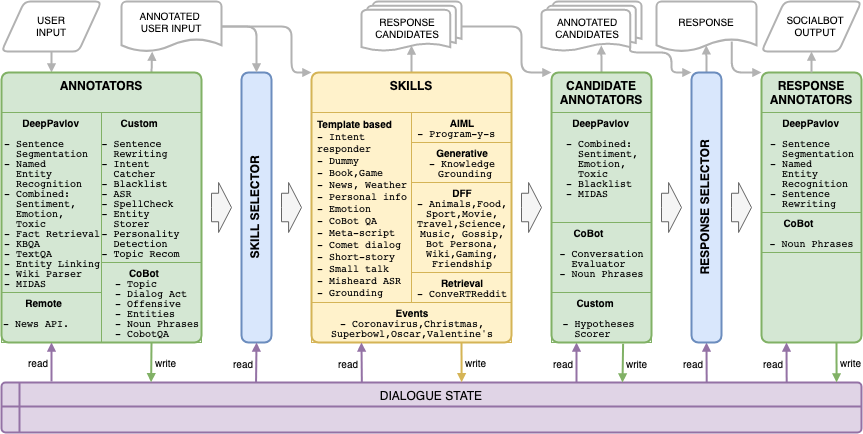
\includegraphics[width=1\linewidth]{images/Alexa2_.png} 
\end{frame}

\begin{frame}{5. Диалоговая платформа DeepPavlov Dream: вклад автора}
\begin{enumerate}
 \item Навыки для обсуждения книг (Book Skill), эмоций (Emotion Skill), сплетен (Gossip Skill, коронавируса (Coronavirus Skill), слухов (Gossip Skill), для обоснования диалога (Grounding Skill), ранжирующий навык TF-IDF (TF-IDF Retrieval), а также генеративный навык, не тестировавшийся на пользователях.
 \item Аннотаторы для классификации эмоций (Emotion Classification), интентов (Intent Catcher), момента остановки диалога (Stop Detect).
 \item Модели для многозадачной классификации (подробнее - в следующих слайдах)
\end{enumerate}
\end{frame}
\begin{frame}{5. Многозадачные модели: зачем нужны ?}
\begin{enumerate}
\item Экономия на вычислительных ресурсах. Стоимость GPU для Dream во время Alexa Prize 4 до 9000\$/мес.
\item Замена удаленных сервисов от Amazon, т.к они были доступны не всегда.
\end{enumerate}
\end{frame}

\begin{frame}{5. Многозадачные модели: с одним линейным слоем}
\begin{enumerate}
\item Замена классификаторов от Amazon (Cobot Topics, Cobot DialogAct Topics, Cobot DialogAct Intents, Cobot Conversation Evaluator), чтобы система Dream могла работать безотносительно политики этой компании.
\item Замена однозадачных классификаторов (Emotion Classification, Sentiment Classification, Toxic Classification) для экономии вычислительных ресурсов.
\end{enumerate}
\begin{table*}[htbp]
\caption{Точность на различных задачах для разных типов однозадачных моделей, в сравнении с многозадачными. }
    \scalebox{0.5}{
    \begin{tabular}{|c|c|c|c|c|} 
    \hline
    \multirow{2}{*}{3адача} & \multicolumn{4}{c|}{Модели} \\
    \cline{2-5}
     & \textbf{Однозадачные} & \textbf{6 в 1} & \textbf{3 в 1 (cobot)} & \textbf{3 в 1 (не cobot)}\\ 
    \hline
    cobot topics   & --- & 84 & 82 & --- \\
    \hline
    cobot dialogact topics  & --- & 76 & 78 & --- \\ 
    \hline
    cobot dialogact intents & --- & 69 & 70 & --- \\ 
    \hline
    Эмоции  & 92 & 82 & --- & 85 \\
    \hline
    Тональность & 72 & 60 & --- & 66 \\ 
    \hline
    Токсичность & 92 & 92 & --- & 93\\ 
    \hline
    \end{tabular}}
\end{table*}
Была выбрана модель "6 в 1".
\scriptsize Также модели с одним линейным слоем применяются для замены модуля оценки диалога от Amazon (Cobot Conversation Evaluator). СКО = 0.31.

\end{frame}


\begin{frame}{5. Многозадачные модели: энкодер-агностичные}
Добавлены новые задачи: 
\begin{enumerate}
    \item Тематическая классификация DeepPavlov Topics.
    \item Классификация фактоидности от YAHOO
    \item Классификация интентов от MIDAS
\end{enumerate}
 Также улучшена предобработка наборов данных для остальных задач, или же была произведена замена наборов данных.
\end{frame}

\begin{frame}{5. Многозадачные энкодер-агностичные модели: результаты}
\begin{table}[htbp]
\caption{Точность моделей в экспериментах с энкодер-агностичными моделями. Для не-Коботовских задач при оценке используются оригинальные тестовые наборы данных, для коботовских -- тестовая часть разбиения данных. «С историей» означает использование диалоговой истории только в задаче MIDAS. «Размер» означает размер обучающей выборки.}
\scalebox{0.6}{
\begin{tabular}{|c|c||c|c|c||c|c|} \hline
Задача & Размер &\begin{tabular}[c]{@{}l@{}}distilbert, S\\с историей\end{tabular} & \begin{tabular}[c]{@{}l@{}}distilbert, M\\с историей\end{tabular}  & \begin{tabular}[c]{@{}l@{}}distilbert, M\\без истории\end{tabular} & \begin{tabular}[c]{@{}l@{}}bert, S\\с историей\end{tabular} & \begin{tabular}[c]{@{}l@{}}bert, M\\с историей\end{tabular}\\ \hline \hline
Эмоции              & 39.5k & \textbf{70.47} & 68.18 & 67.59 & \textbf{71.48} & 67.27\\ \hline
Токсичность            & 162k & \textbf{94.53} & 93.84 & 93.86         & \textbf{94.54} & 93.94 \\ \hline
Тональность            & 94k  & \textbf{74.75} & 72.55 & 72.22  & \textbf{75.95} & 75.65 \\ \hline
Интенты MIDAS          & 7.1k & \textbf{80.53} & 72.73 & 73.69 & \textbf{82.3}  & 77.01 \\ \hline
Фактоидность            & 3.6k & \textbf{81.69} & 81.02 & 80.0 & \textbf{84.41} & 80.34 \\ \hline
DeepPavlov Topics & 1.8M & \textbf{87.48} & 86.98  & 87.01  & \textbf{88.09}  & 87.43\\ \hline
cobot topics                   & 216k & \textbf{79.88}  & 77.31 & 77.45         & \textbf{80.68} & 78.21 \\ \hline
\begin{tabular}[c]{@{}l@{}}cobot dialogact\\ topics \end{tabular}            & 127k & 76.81 & \textbf{76.92} & 76.8   & \textbf{77.02} & 76.86 \\ \hline
\begin{tabular}[c]{@{}l@{}}cobot dialogact \\intents \end{tabular}           & 318k & \textbf{77.07}  & 76.83 & 76.65         & \textbf{77.28} & 76.96 \\ \hline
Средее для 9 задач                   & 2.76M & \textbf{80.36}    & 78.48 & 78.36        & \textbf{81.31}  & 79.3 \\ \hline
\begin{tabular}[c]{@{}l@{}} Видеопамяти \\ использовано, Мб    \end{tabular}            &    & 2418*9=21762 & \textbf{2420}     & \textbf{2420}             & 3499*9=31491 & \textbf{3501}    \\ \hline
\end{tabular}
}
\end{table}
Многозадачные модели требуют в 9 раз меньше памяти, чем однозадачные, при этом почти не хуже. Был выбран \textbf{distilbert, M без истории}.
\end{frame}
\begin{frame}{5. Многозадачные энкодер-агностичные модели: сравнение с моделями с одним линейным слоем}
\begin{table}[htbp]
\centering
\caption {\small Точность моделей в экспериментах с многозадачными моделями.  «Новая» означает энкодер-агностичную модель, «Старая» - модель с одним линейным слоем. Все модели основаны на \textit{distilbert-base-uncased}, история только в наборе данных MIDAS.% Для не-Коботовских задач при оценке используются оригинальные тестовые наборы данных, для коботовских -- тестовая часть разбиения данных. «Размер» означает размер обучающей выборки.
}
\label{tab:tr-ag-dream2}% label всегда желательно идти после caption
\scalebox{0.5}{
\begin{tabular}{|c||c|c|c|c|} \hline
\multirow{4}{*}{Задача}  &Новая & Старая & Старая & Старая \\
 & &             & мягкие & дополненные \\
 & & независимые & независимые & независимые \\
 & & метки & метки & метки \\ \hline \hline
Эмоции               & 68.18 & 66.2 & 57.57 & \textbf{70.14} \\ \hline
Токсичность              & 93.84  & 93.74 & 93.79 & \textbf{94.54} \\ \hline
Тональность               & 72.55 & 71.47 & 70.81 & \textbf{74.59} \\ \hline
Интенты MIDAS            & 72.73 & \textbf{74.55} & 30.54 & 74.37 \\ \hline
Фактоидность           & 81.02 & 79.6 & 69.02 & \textbf{81.61} \\ \hline
DeepPavlov Topics  & \textbf{86.98} & 86.39 & 86.66 & 86.93 \\ \hline
cobot topics  & 77.31 & 60.03 & 34.22 & 78.6 \\ \hline
\begin{tabular}[c]{@{}l@{}}cobot dialogact\\ topics \end{tabular}              & \textbf{76.92} & 71.17 & 66.43 & 73.56\\ \hline
\begin{tabular}[c]{@{}l@{}}cobot dialogact \\intents \end{tabular}            & {76.83} & 76.2 & 76.47 & \textbf{77.27} \\ \hline
Среднее для 9 задач                  & {78.48} & 75.48 & 65.06 & \textbf{79.07} \\ \hline
\end{tabular}
}
\end{table}
{\small Старая хуже новой, если не делать псевдоразметку однозадачными моделями. Если сложная задача и много классов - сильно хуже. \newline
Только если сильно увеличить датасеты за счёт такой псевдоразметки, модель с одним линейным слоем чуточку лучше. }
\end{frame}


\begin{frame}{Научная новизна}
\begin{enumerate}
  \item {Впервые получена оценка влияния различных методов псевдоразметки данных на качество многозадачных моделей. Выделен тип задач, для которых объединение меток при многозадачной классификации оправдано.}
  \item {Впервые получена  оценка зависимости качества  работы энкодер-агностичных многозадачных нейросетевых моделей на диалоговых задачах из различных языков от размера обучающей выборки, в том числе при переносе знаний между языками.}
  \item {Впервые для дообучения на русском языке получена оценка зависимости межъязыкового переноса знаний на разговорных данных в многоязычных нейросетевых моделях от размера предобучающей выборки и генеалогической близости языков к языку дообучения.}
  %\item {Впервые получена оценка качества работы различных оригинальных многозадачных нейросетевых архитектур и методов псевдоразметки данных на задачах диалоговой платформы Dream.}
\end{enumerate}    
\end{frame}

\begin{frame}
    \frametitle{Положения, выносимые на защиту}
    \begin{enumerate}
  \item {Псевдоразметка данных с использованием однозадачных моделей улучшает метрики многозадачных моделей. При этом объединение классов оправдано только для задач, достаточно сильно похожих друг на друга.}
  \item {Для достаточно малых данных многозадачные энкодер-агностичные модели превосходят по своей средней точности однозадачные, в особенности -- за счет задач с наименьшим объемом данных. При этом для таких многоязычных моделей наблюдается также перенос знаний с английского языка на русский в рамках одной задачи, и чем меньше русскоязычных данных, тем сильнее выражен перенос. Эта закономерность справедлива и для однозадачных моделей.}
  \item {Для многоязычных нейросетевых моделей качество переноса знаний на разные языки на тематических данных сильно коррелирует с размером предобучающей выборки для каждого языка, но при этом после поправки на размер предобучающей выборки статистически значимая корреляция с генеалогической близостью этого языка к языку дообучения не обнаруживается.}
    \end{enumerate}
\end{frame}

\begin{frame}{Практическая значимость}
\begin{enumerate}
   \item { Был создан ряд компонент диалоговой платформы мирового уровня, впервые в России вышедшей в полуфинал престижных мировых конкурсов Alexa Prize 3 и Alexa Prize 4. В число этих компонент входят многозадачные нейросетевые модели: многозадачная нейросетевая модель с одним линейным слоем, многозадачная нейросетевая модель на основе архитектуры PAL-BERT и многозадачная энкодер-агностичная нейросетевая модель. Диалоговая платформа имеет полностью открытый код, что дает возможность легкого переиспользования любой части проделанной над ней работы. При этом многозадачная энкодер-агностичная модель даёт на девяти задачах данной диалоговой платформы экономию видеопамяти $\sim$90\% и экономию оперативной памяти $\sim$79\% по сравнению с аналогичными однозадачными моделями, даже не учитывая эффект от возможности быстрой замены базовой модели.}
\end{enumerate}    
\end{frame}
\begin{frame}{Практическая значимость}
\begin{enumerate}
\setcounter{enumi}{1}
   \item {Программный код для реализации многозадачной энкодер-агностичной нейросетевой модели встроен в библиотеку DeepPavlov, имевшую более 500000 скачиваний на момент встраивания кода. Данные модели позволяют решить большое число задач без дополнительных вычислительных затрат, не считая затрат на использование задаче-специфичных линейных слоёв (всего $\sim$0.1\% дополнительных параметров для решения сразу пяти задач вместо одной)}
\end{enumerate}    
\end{frame}

\begin{frame}{Основные публикации}
 Основные результаты по теме диссертации изложены в 8~публикациях, {1} из которых издано в журналах, рекомендованных ВАК, {1} в~периодических научных журналах, индексируемых Web of~Science и Scopus (еще 2 - принято в такие журналы и готовится к публикации), {4} в~тезисах докладов.\footnote{Цифры будут уточнены после принятия всех статей.} Получен также 1 патент.
 \newline
\begin{enumerate}
 \item Karpov, D. Data pseudo-labeling while adapting BERT for multitask
approaches  / D. Karpov, M. Burtsev // Komp’juternaja
Lingvistika i Intellektual’nye Tehnologii. — 2021. — С. 358—366.
\item  Karpov, D. Knowledge Transfer in the Multi-task Transformer-agnostic
Models On Conversational Tasks (готовится к публикации) /
D. Karpov, V. Konovalov // Proceedings of the International Conference
«Dialogue 2023». — 2023.
\item Karpov, D. Monolingual and Cross-Lingual Knowledge Transfer for
Topic Classification (готовится к публикации)/ D. Karpov,
M. Burtsev // Proceedings of AINL 2023. — 2023.
\end{enumerate}
\end{frame}

\begin{frame}{Основные публикации}
\begin{enumerate}
\setcounter{enumi}{3}
\item Dream technical report for the Alexa Prize 2019 / Y. Kuratov
[и др.] // 3rd Proc. Alexa Prize. — 2019.
\item Dream technical report for the Alexa Prize 4  / D. Baymurzina
[и др.] // 4th Proc. Alexa Prize. — 2021.
\item Юсупов И.Ф. и Баймурзина Д.Р. и Кузнецов Д.П. и Чернявский Д.В. и Дмитриевский А. и Ермакова Е.С. и Игнатов Ф.С. и Карпов Д.А. и Корнев Д.А. и Ли Т.А. и Пугин П.Ю. и Бурцев М.С. Диалоговая система Dream в конкурсе Alexa
Prize Challenge 2019 // Труды Московского физико-технического
института. — 2021. — Т. 13, 3 (51). — С. 62—89
\end{enumerate}
\end{frame}
\begin{frame}{Основные публикации}
\begin{enumerate}
\setcounter{enumi}{6}
\item DeepPavlov Dream: Platform for Building Multiskill Generative Assistants (готовится к публикации) / Dilyara Zharikova, Daniel Kornev, Fedor Ignatov, Maxim Talimanchuk, Dmitry Evseev, Ksenya Petukhova, Veronika Smilga, Dmitry Karpov, Yana Shishkina, Dmitry Kosenko and Mikhail Burtsev / Proceedings of the ACL Systems Demo, 2023
\item Разработка диалоговой системы с интеграцией профиля лично
сти  / Д. Болотин, Д. Карпов [и др.] //. 5th International Conference
on Engineering and Telecommunication EnT—MIPT 2018. — MIPT,
2019. — URL: http://2019.en-t.info/old/articles/ent2018-thesis.pdf ;
Конференция проходила 15-16 декабря 2018 года. Место проведения:
Москва/Долгопрудный/«Физтехпарк».
\item Свидетельство о депонировании, Texter ocr-cv-nlp-microservice / В. Дуплякин, А. Ондар, Д. Карпов, А. Ушаков — 2021.
\end{enumerate}    
\end{frame}

\begin{frame}{.}
\centering
\Large \textbf{Спасибо за внимание!}
\end{frame}
\iffalse
\fi
